\documentclass[journal,12pt,twocolumn]{IEEEtran}

\usepackage{setspace}
\usepackage{gensymb}
\singlespacing
\usepackage[cmex10]{amsmath}

\usepackage{amsthm}

\usepackage{mathrsfs}
\usepackage{txfonts}
\usepackage{stfloats}
\usepackage{bm}
\usepackage{cite}
\usepackage{cases}
\usepackage{subfig}

\usepackage{longtable}
\usepackage{multirow}

\usepackage{enumitem}
\usepackage{mathtools}
\usepackage{steinmetz}
\usepackage{tikz}
\usepackage{circuitikz}
\usepackage{verbatim}
\usepackage{tfrupee}
\usepackage[breaklinks=true]{hyperref}
\usepackage{graphicx}
\usepackage{tkz-euclide}

\usetikzlibrary{calc,math}
\usepackage{listings}
    \usepackage{color}                                            %%
    \usepackage{array}                                            %%
    \usepackage{longtable}                                        %%
    \usepackage{calc}                                             %%
    \usepackage{multirow}                                         %%
    \usepackage{hhline}                                           %%
    \usepackage{ifthen}                                           %%
    \usepackage{lscape}     
\usepackage{multicol}
\usepackage{chngcntr}

\DeclareMathOperator*{\Res}{Res}

\renewcommand\thesection{\arabic{section}}
\renewcommand\thesubsection{\thesection.\arabic{subsection}}
\renewcommand\thesubsubsection{\thesubsection.\arabic{subsubsection}}

\renewcommand\thesectiondis{\arabic{section}}
\renewcommand\thesubsectiondis{\thesectiondis.\arabic{subsection}}
\renewcommand\thesubsubsectiondis{\thesubsectiondis.\arabic{subsubsection}}


\hyphenation{op-tical net-works semi-conduc-tor}
\def\inputGnumericTable{}                                 %%

\lstset{
%language=C,
frame=single, 
breaklines=true,
columns=fullflexible
}
\begin{document}

\newcommand{\BEQA}{\begin{eqnarray}}
        \newcommand{\EEQA}{\end{eqnarray}}
\newcommand{\define}{\stackrel{\triangle}{=}}
\bibliographystyle{IEEEtran}
\raggedbottom
\setlength{\parindent}{0pt}
\providecommand{\mbf}{\mathbf}
\providecommand{\pr}[1]{\ensuremath{\Pr\left(#1\right)}}
\providecommand{\qfunc}[1]{\ensuremath{Q\left(#1\right)}}
\providecommand{\sbrak}[1]{\ensuremath{{}\left[#1\right]}}
\providecommand{\lsbrak}[1]{\ensuremath{{}\left[#1\right.}}
\providecommand{\rsbrak}[1]{\ensuremath{{}\left.#1\right]}}
\providecommand{\brak}[1]{\ensuremath{\left(#1\right)}}
\providecommand{\lbrak}[1]{\ensuremath{\left(#1\right.}}
\providecommand{\rbrak}[1]{\ensuremath{\left.#1\right)}}
\providecommand{\cbrak}[1]{\ensuremath{\left\{#1\right\}}}
\providecommand{\lcbrak}[1]{\ensuremath{\left\{#1\right.}}
\providecommand{\rcbrak}[1]{\ensuremath{\left.#1\right\}}}
\theoremstyle{remark}
\newtheorem{rem}{Remark}
\newcommand{\sgn}{\mathop{\mathrm{sgn}}}
\providecommand{\abs}[1]{\vert#1\vert}
\providecommand{\res}[1]{\Res\displaylimits_{#1}}
\providecommand{\norm}[1]{\lVert#1\rVert}
%\providecommand{\norm}[1]{\lVert#1\rVert}
\providecommand{\mtx}[1]{\mathbf{#1}}
\providecommand{\mean}[1]{E[#1]}
\providecommand{\fourier}{\overset{\mathcal{F}}{ \rightleftharpoons}}
%\providecommand{\hilbert}{\overset{\mathcal{H}}{ \rightleftharpoons}}
\providecommand{\system}{\overset{\mathcal{H}}{ \longleftrightarrow}}
%\newcommand{\solution}[2]{\textbf{Solution:}{#1}}
\newcommand{\solution}{\noindent \textbf{Solution: }}
\newcommand{\cosec}{\,\text{cosec}\,}
\providecommand{\dec}[2]{\ensuremath{\overset{#1}{\underset{#2}{\gtrless}}}}
\newcommand{\myvec}[1]{\ensuremath{\begin{pmatrix}#1\end{pmatrix}}}
\newcommand{\mydet}[1]{\ensuremath{\begin{vmatrix}#1\end{vmatrix}}}
\numberwithin{equation}{subsection}
\makeatletter
\@addtoreset{figure}{problem}
\makeatother
\let\StandardTheFigure\thefigure
\let\vec\mathbf
\renewcommand{\thefigure}{\theproblem}
\def\putbox#1#2#3{\makebox[0in][l]{\makebox[#1][l]{}\raisebox{\baselineskip}[0in][0in]{\raisebox{#2}[0in][0in]{#3}}}}
\def\rightbox#1{\makebox[0in][r]{#1}}
\def\centbox#1{\makebox[0in]{#1}}
\def\topbox#1{\raisebox{-\baselineskip}[0in][0in]{#1}}
\def\midbox#1{\raisebox{-0.5\baselineskip}[0in][0in]{#1}}
\vspace{3cm}
\title{AI1103 Assignment-1}
\author{SRIVATSAN T - CS20BTECH11062}
\maketitle
\newpage
\bigskip
\renewcommand{\thefigure}{\theenumi}
\renewcommand{\thetable}{\theenumi}
Download all python codes from
\begin{lstlisting}
https://github.com/CS20BTECH11062/AI1103/tree/main/Assignment-3/codes
\end{lstlisting}
%
and latex-tikz codes from
%
\begin{lstlisting}
https://github.com/CS20BTECH11062/AI1103/tree/main/Assignment-3/Assignment-3.tex
\end{lstlisting}
\section*{QUESTION (GATE-MA-2014-36)}
The time to failure, in months, of lights bulbs \\manufactured at two plants A and B
obey the exponential distributions with means 6 and 2 months respectively. Plant B produces
four times as many bulbs as plant A does. Bulbs from these two plants are indistinguishable.
They are mixed and sold together. Given that a bulb purchased at random is working after 12 months, What is the probability that it was manufactured in plant A?
\section*{SOLUTION}
Given that 90 \% of the population is 'right' handed and since being 'right' handed and being 'left' handed are mutually exclusive,
\bigskip
\begin{itemize}
    \item Probability of 'right' handed = $\pr{R}$ = \(\frac{9}{10}\)
    \item Probability of 'left' handed = $\pr{L}$ = \( \frac{1}{10} \)
\end{itemize}
\bigskip
One can use binomial distribution to find out the probability that more that 6 people are 'right' handed.\\
Let M be a variable representing number of people who are 'right' handed in a given sample.\\
So M has a binomial distribution :
\begin{align}
    \pr{M=k} = {{n}\choose{k}} \times (l)^{n-k} \times (r)^{k}\label{0.0.1}
\end{align}
Where
\begin{itemize}
    \item n = Total number of people = 10
    \item l = Probability that a person is 'left' handed = \( \frac{1}{10} \)
    \item r = Probability that a person is 'right' handed = \( \frac{9}{10} \)
\end{itemize}
\bigskip
So,
\begin{align}
    \pr{M=k} = {{n}\choose{k}} \times \brak{\frac{1}{10}}^{n-k} \times \brak{\frac{9}{10}}^{k}\label{0.0.2}
\end{align}
\begin{center}
    $\Pr$(at most 6 are right handed) = $\pr{M = 0}$\\+ $\pr{M = 1}$ + $\pr{M = 2}$ + $\pr{M = 3}$ \\+ $\pr{M = 4}$ + $\pr{M = 5}$ + $\pr{M = 6}$\\
\end{center}
\begin{align}
    \implies \pr{0\leq M \leq 6} = 1 - \pr{7 \leq M \leq10}\label{0.0.3}
\end{align}
\begin{center}
    (Since $\sum_{k=0}^{10}$ $\pr{M=k}$ = 1)\\
\end{center}
\begin{align}
    \implies 1 - \pr{7 \leq M \leq 10} = 1 - \sum_{k=7}^{10} \pr{M=k}\label{0.0.4}
\end{align}
From \eqref{0.0.2} we get,
\begin{align}
    \implies 1 - \sum_{k=7}^{10} {{10}\choose{k}} \times \brak{\frac{1}{10}}^{10-k} \times \brak{\frac{9}{10}}^{k}\label{0.0.5}
\end{align}

\begin{align}
    \begin{split}
        \implies 1 - {{10}\choose{7}} \times \brak{\frac{1}{10}}^{3} \times \brak{\frac{9}{10}}^{7} - {{10}\choose{8}} \times \brak{\frac{1}{10}}^{2} \times \brak{\frac{9}{10}}^{8}
        \bigskip\\
        -{{10}\choose{9}} \times \brak{\frac{1}{10}}^{1} \times \brak{\frac{9}{10}}^{9} - {{10}\choose{10}} \times \brak{\frac{1}{10}}^{0}\times
        \brak{\frac{9}{10}}^{10}\label{0.0.6}
    \end{split}
\end{align}
\begin{align}
    \implies \pr{0 \leq M \leq 6} = \frac{7996999}{625000000} = 0.012795198\notag
\end{align}

\bigskip
Thus the probability that at most 6 people are 'right' handed is 0.012795198
\pagebreak
%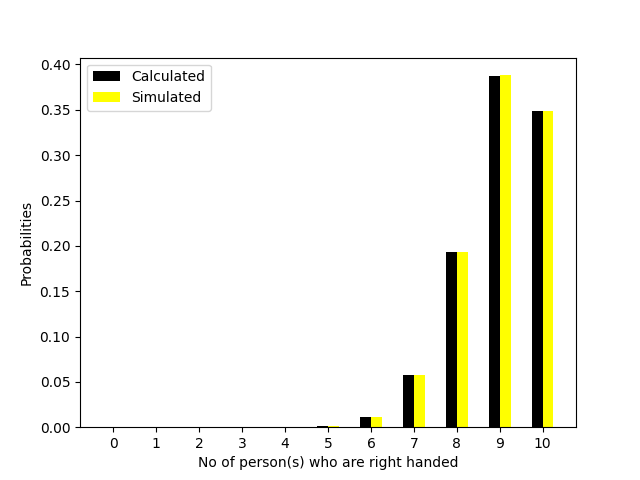
\includegraphics{Figure-1.png}
\end{document}